\documentclass[11pt]{article}
\usepackage[margin=1in]{geometry}
\usepackage{amsmath}
\usepackage{booktabs}
\usepackage{graphicx}
\usepackage{circuitikz}
\definecolor{hl}{HTML}{EA580C}
\usepackage[hidelinks]{hyperref}
\usepackage{parskip}

\newcommand{\Vdet}{V_{\mathrm{det}}}
\newcommand{\Venv}{V_{\mathrm{env}}}
\newcommand{\Vbe}{V_{\mathrm{BE}}}
\newcommand{\Rtop}{R_{\mathrm{top}}}
\newcommand{\Rbot}{R_{\mathrm{bot}}}
\newcommand{\kO}{\,\mathrm{k\Omega}}

\title{Audio Visualizer: Sizing the LED Loudness Ladder}
\author{Lucas Krippendorff}
\date{}

\begin{document}
\maketitle

\noindent
Ten LEDs per channel that light in sequence with loudness. No driver IC,
just transistors, resistors, and half an LM358 per channel. This is the math
behind the resistor values.

\begin{figure}[h]
\centering
\begin{circuitikz}[american, scale=0.82, transform shape]
  % envelope detector
  \draw (0,0) node[left]{audio in} to[C, l=$1\,\mu$F] (1.9,0) to[D, l=BAT85] (3.5,0);
  \draw (3.5,0) node[circ]{} node[above=4pt, xshift=8pt]{$\Vdet$};
  \draw (3.5,0) to[C, l_=$10\,\mu$F] (3.5,-2.2) node[ground]{};
  \draw (3.5,0) -- (5.1,0);
  \draw (5.1,0) node[circ]{} to[R, l_=22k] (5.1,-2.2) node[ground]{};
  % op amp, non-inverting x2.1 (flipped: + on top, feedback below)
  \node[op amp, noinv input up, anchor=+] (oa) at (8.1,0) {};
  \node[above=1pt] at (oa.north) {LM358};
  \draw (5.1,0) -- (oa.+);
  \draw (oa.-) -- ++(-0.4,0) coordinate(fb) -- ++(0,-0.9) coordinate(fb3) node[circ]{};
  \draw (fb3) to[R, l_=10k] ++(0,-1.6) node[ground]{};
  \draw (oa.out) -- ++(0.4,0) coordinate(o1) node[circ]{};
  \draw (fb3) to[R, l_=11k] (fb3 -| o1) -- (o1);
  \draw (o1) to[short, -*] ++(0.7,0) coordinate(bus) node[above=2pt]{$\Venv$};
  % divider + stage
  \draw (bus) to[R, l=$R_{\mathrm{top},k}$] ++(2.5,0) coordinate(b) node[circ]{};
  \node[above=4pt, xshift=6pt, color=hl] at (b) {$\Vbe$};
  \draw (b) to[R, l_=$R_k$] ++(0,-2.2) node[ground]{};
  \draw (b) -- ++(0.8,0) node[npn, anchor=B] (q) {};
  \node[right=6pt, yshift=-10pt] at (q.east) {MMBT3904};
  \draw (q.E) -- ++(0,-0.3) node[ground]{};
  \draw (q.C) ++(0,3.2) node[vcc]{+12\,V} to[R, l=3.3k] ++(0,-1.7) to[full led, l=LED] (q.C);
\end{circuitikz}
\caption{Front end and one of ten ladder stages (one channel of two). The
divider pair $R_{\mathrm{top},k}$/$R_k$ changes from stage to stage. LED $k$
turns on when its base hits $\Vbe$; the threshold $V_k$ is not a node, just
the $\Venv$ value that gets the base there.}
\end{figure}

\section*{Getting a loudness voltage}

Audio is AC; the ladder needs a DC voltage that tracks volume. A $1\,\mu$F cap
couples the signal in, a Schottky rectifies it, a $10\,\mu$F cap holds the
peak, and a $22\kO$ bleed lets it fall
($\tau = 22\kO \times 10\,\mu\mathrm{F} \approx 0.22$\,s). That's $\Vdet$.

I call $\Vdet = 5$\,V clipping. That's an educated guess: the speakers can
theoretically swing 6\,V, but the Schottky eats $\sim$0.3\,V right after the
coupling cap and the other parts in series take their share. This display is
purely cosmetic, so being off by a little here costs nothing. 5\,V it was.

\section*{Log spacing, because hearing is logarithmic}

Equal steps in perceived loudness are equal voltage \emph{ratios}, not equal
volts. So the thresholds are spaced in dB, the same call the LM3915 bar
driver this circuit replaces makes. 30\,dB of range, 13 steps, 2.5\,dB each:
\begin{equation}
L_k = -30 + 2.5\,(k-1)\ \mathrm{dB}, \qquad
V_k = V_{\mathrm{fs}} \cdot 10^{L_k/20}.
\end{equation}

\section*{Filling the 12\,V rail}

The detector tops out at 5\,V but the board runs on 12. An LM358 on a 12\,V
rail can only swing to about 10.5\,V, so I picked the gain to land full scale
exactly there: $A = 10.5/5 = 2.1$, built as $1 + 11\mathrm{k}/10\mathrm{k}$.
Full scale and clipping are the same voltage on purpose, which makes the top
LED the clip light. The op amp also buffers the detector: the ladder pulls
its current from the op amp instead of draining the peak-hold cap.

\section*{One transistor, three resistors per LED}

Each stage is an NPN with a grounded emitter and an LED with its $3.3\kO$
current limiter on the collector. Two more resistors form the base divider
that decides when the stage turns on:
\begin{equation}
V_k = \Vbe\left(1 + \frac{\Rtop}{R_k}\right)
\quad\Longrightarrow\quad
\frac{\Rtop}{R_k} = \frac{V_k}{\Vbe} - 1.
\label{eq:rk}
\end{equation}
A divider can only divide, so nothing below $\Vbe \approx 0.65$\,V is
reachable. Any division under that line simply can't be built. The 13 came
from trial and error: with 13 divisions, exactly three (0.33, 0.44,
0.59\,V) fall under $\Vbe$, and the 10 LEDs I wanted survive. Usable range:
$-22.5$ to 0\,dB.

My first pass fixed $\Rtop = 10\kO$ everywhere: one resistor to calculate
per LED, about a milliamp per divider at full scale. Then the JLCPCB order
got real. It's not enough for a value to exist as a standard E24 part; it
also has to be in JLCPCB's \emph{basic} catalog, because every unique
extended part adds a loading fee to assembly, and several of the
10k-anchored values were extended only. Since the divider only cares about
the ratio in Eq.~\eqref{eq:rk}, I re-picked both resistors per stage from
the basic catalog. Dividers stay in the same roughly-a-milliamp range, and
the errors actually improved: worst case fell from 3.8\% to 1.4\%. The error
column is how far the built threshold lands from the ideal $V_k$; adjacent
thresholds are 33\% apart, so turn-on order was never in danger:

\begin{center}
\begin{tabular}{c r r r r r r}
\toprule
LED & $L_k$ & ideal $V_k$ & $\Rtop$ & $R_k$ & threshold & error \\
\midrule
1  & $-22.5$\,dB & 0.787\,V  & $10\kO$  & $47\kO$  & 0.788\,V  & $+0.1\%$ \\
2  & $-20.0$\,dB & 1.050\,V  & $20\kO$  & $33\kO$  & 1.044\,V  & $-0.6\%$ \\
3  & $-17.5$\,dB & 1.400\,V  & $27\kO$  & $24\kO$  & 1.381\,V  & $-1.4\%$ \\
4  & $-15.0$\,dB & 1.867\,V  & $22\kO$  & $12\kO$  & 1.842\,V  & $-1.4\%$ \\
5  & $-12.5$\,dB & 2.490\,V  & $6.8\kO$ & $2.4\kO$ & 2.492\,V  & $+0.1\%$ \\
6  & $-10.0$\,dB & 3.320\,V  & $10\kO$  & $2.4\kO$ & 3.358\,V  & $+1.1\%$ \\
7  & $-7.5$\,dB  & 4.428\,V  & $27\kO$  & $4.7\kO$ & 4.384\,V  & $-1.0\%$ \\
8  & $-5.0$\,dB  & 5.905\,V  & $22\kO$  & $2.7\kO$ & 5.946\,V  & $+0.7\%$ \\
9  & $-2.5$\,dB  & 7.874\,V  & $30\kO$  & $2.7\kO$ & 7.872\,V  & $-0.0\%$ \\
10 & $0.0$\,dB   & 10.500\,V & $15\kO$  & $1\kO$   & 10.400\,V & $-1.0\%$ \\
\bottomrule
\end{tabular}
\end{center}

Collector resistors:
$R_C = (12 - 2.0 - 0.2)\,\mathrm{V} / 3\,\mathrm{mA} \approx 3.3\kO$ per LED.
The board carries two identical channels, left and right.

\begin{figure}[h]
\centering
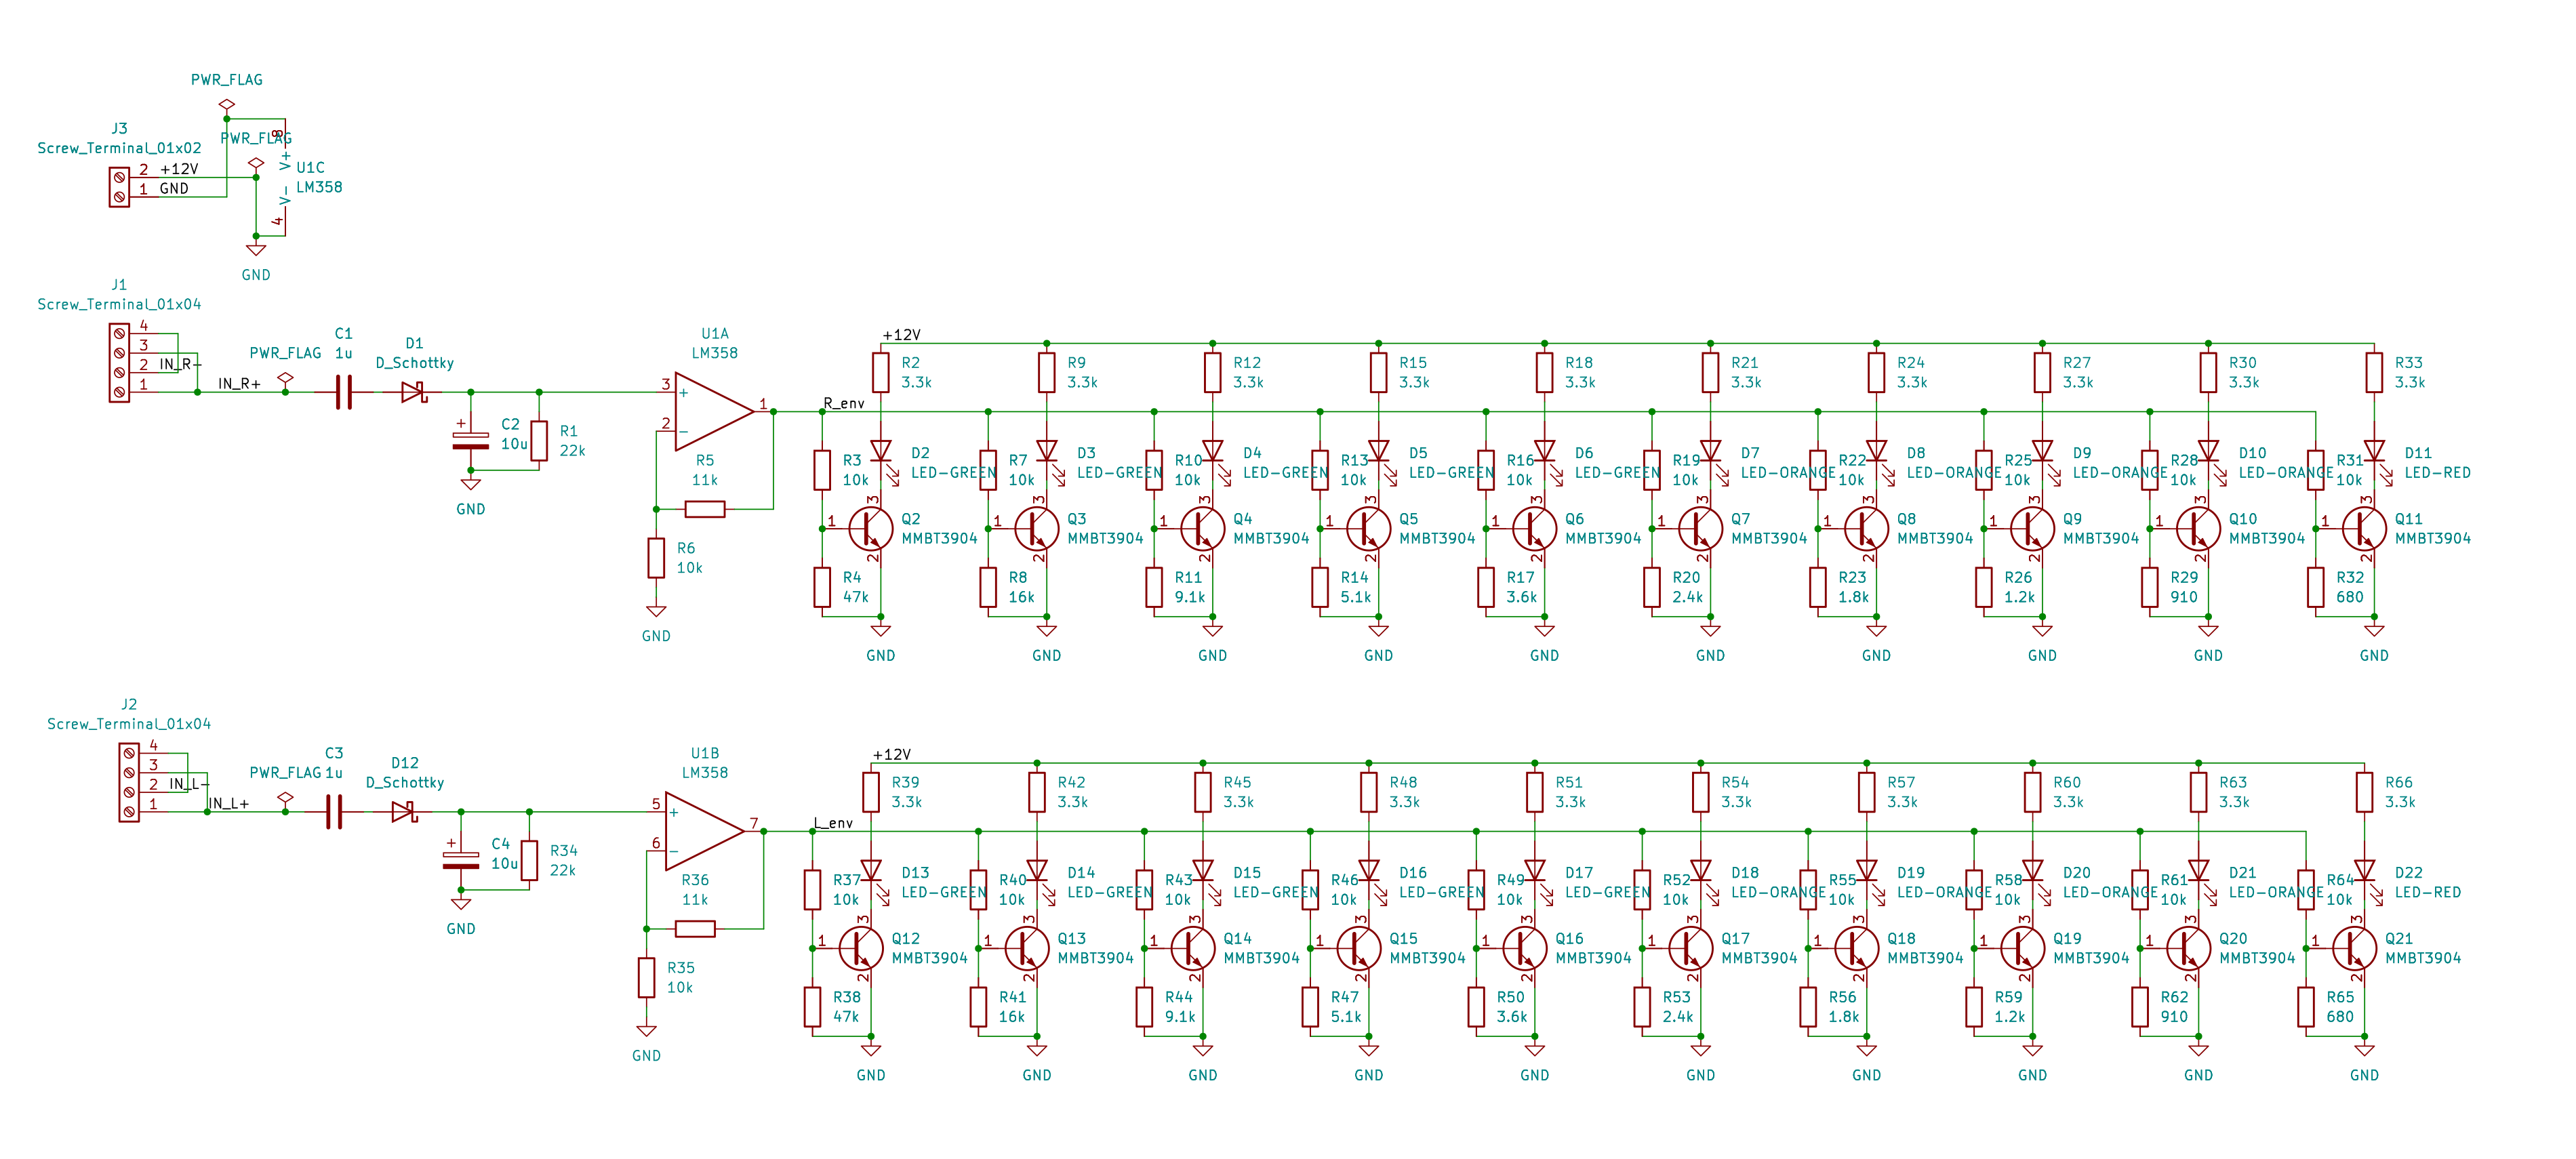
\includegraphics[width=\textwidth]{schematic_kicad.png}
\caption{Full schematic: both channels, each half of the LM358 driving its
own ten-stage ladder.}
\end{figure}

\begin{figure}[h]
\centering
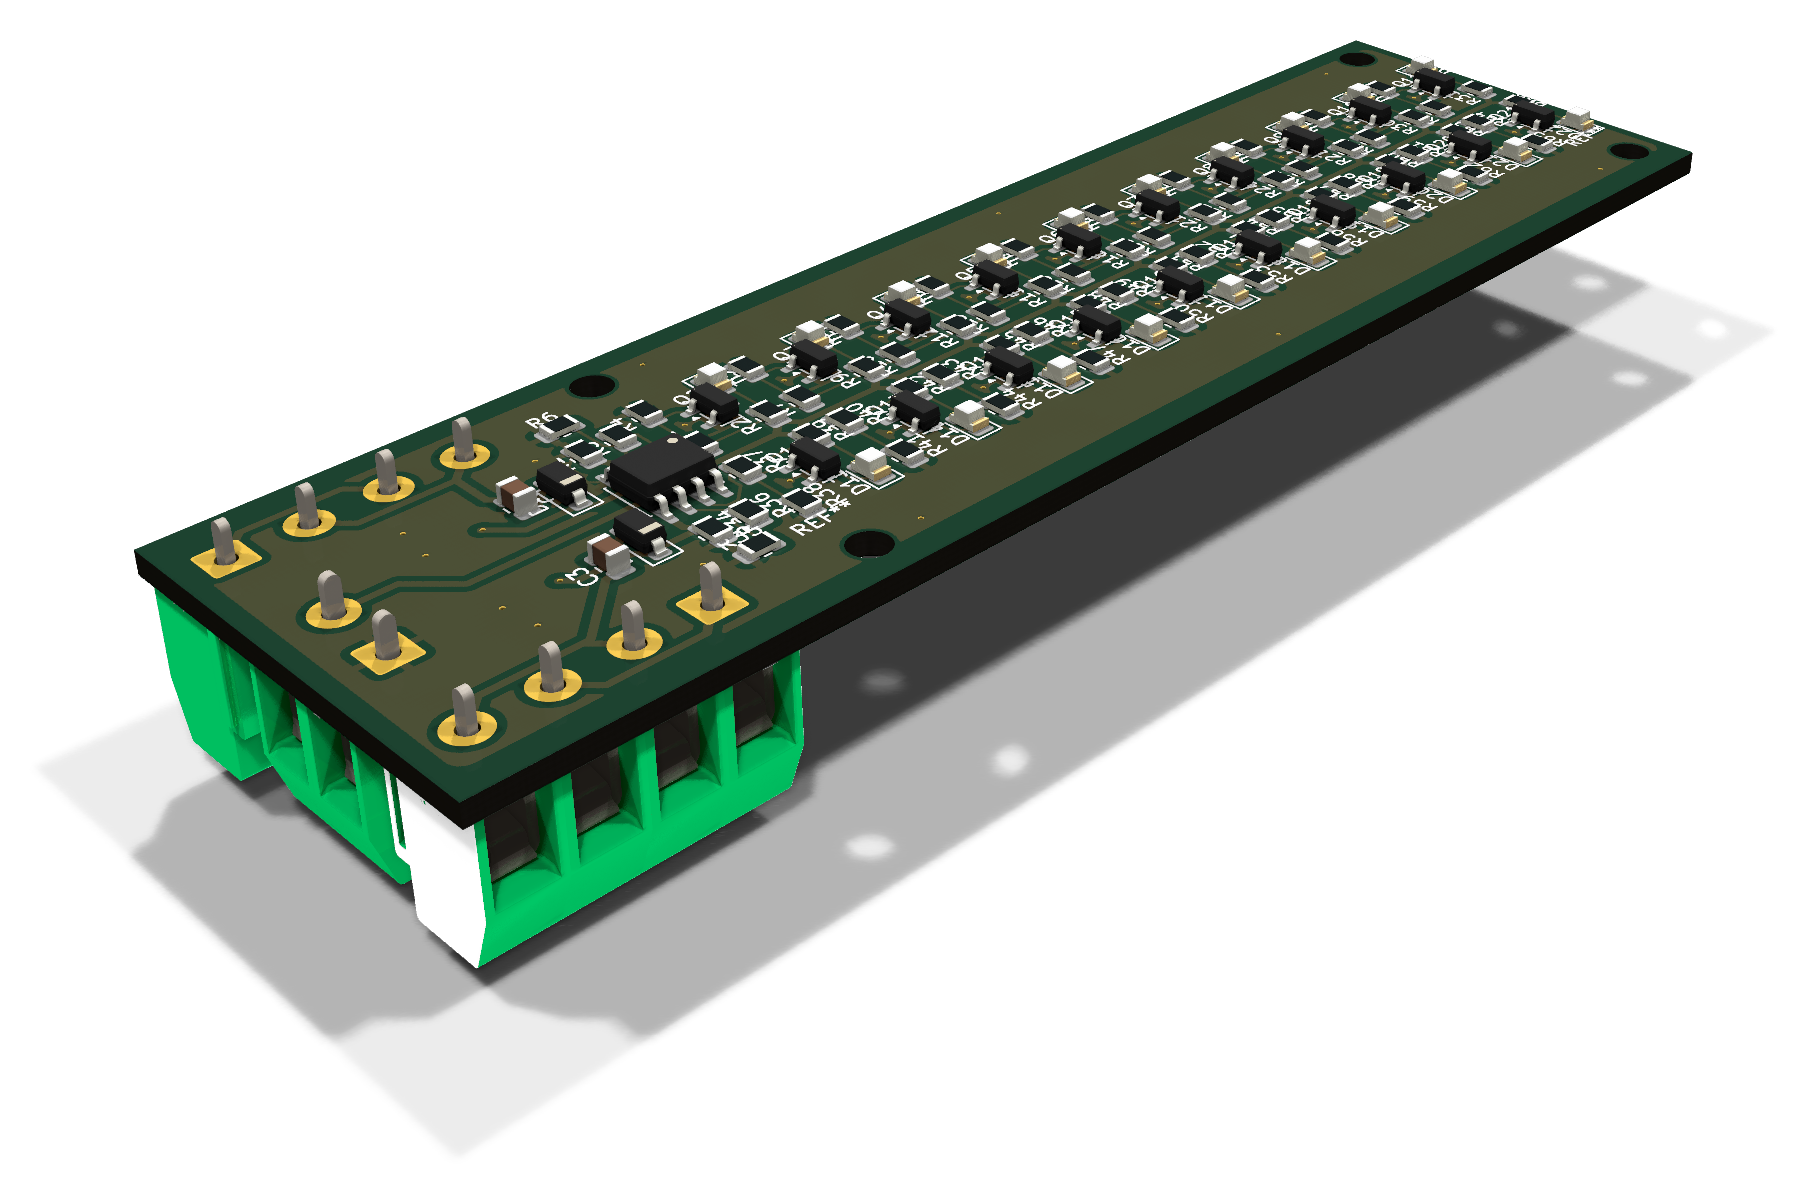
\includegraphics[width=0.62\textwidth]{render_corner.png}\\[6pt]
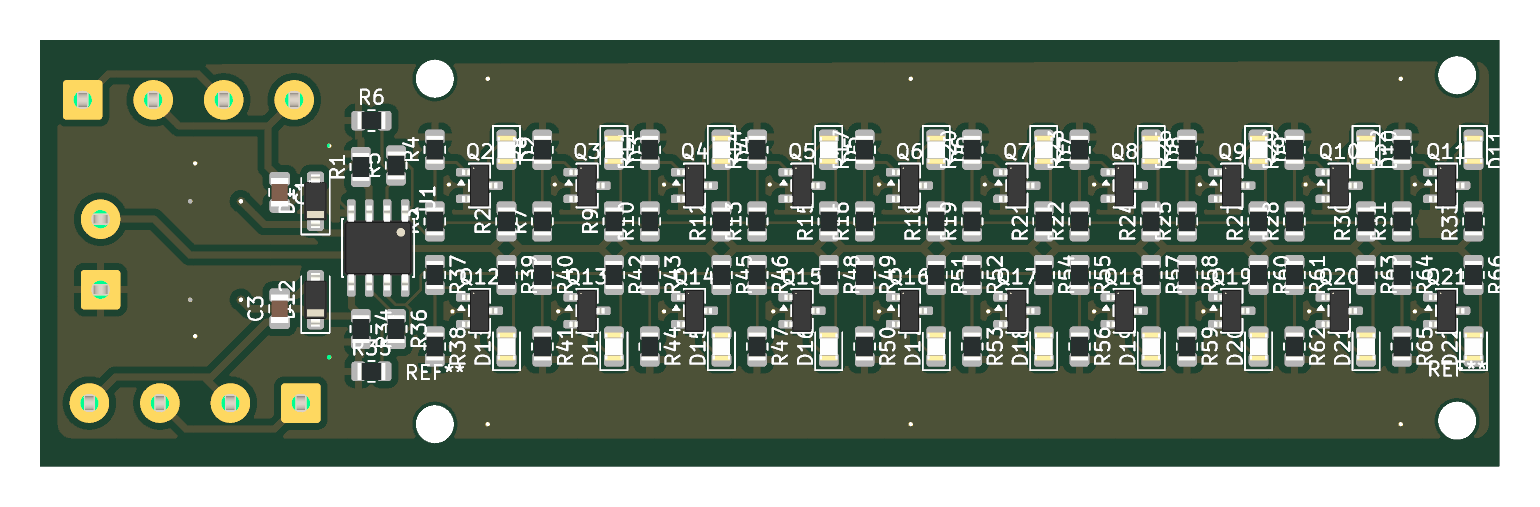
\includegraphics[width=0.85\textwidth]{render_top.png}
\caption{V1 board: two 10-LED channels, MMBT3904 ladder, LM358 front end.}
\end{figure}

\end{document}
